% RestoreNet report. NeurIPS-STYLE layout approximated with standard packages because the official
% neurips_20XX.sty cannot be bundled/downloaded here. To use the official style: put neurips_20XX.sty next to
% this file, delete the "approximate NeurIPS layout" block below and add \usepackage{neurips_20XX}.
% All numbers in the prose come from \newcommand{\ColorizerName}{Zhang2016-pretrained (deep, Caffe via OpenCV DNN)}
\newcommand{\ColorizerKind}{deep}
\newcommand{\NImages}{4}
\newcommand{\mDegPsnrGray}{19.03}
\newcommand{\mDegSsimGray}{0.46}
\newcommand{\mClsPsnrGray}{19.24}
\newcommand{\mClsSsimGray}{0.58}
\newcommand{\mAPsnrGray}{19.05}
\newcommand{\mASsimGray}{0.46}
\newcommand{\mAPsnrRgb}{17.14}
\newcommand{\mASsimRgb}{0.42}
\newcommand{\mAAbRmse}{21.09}
\newcommand{\mBPsnrGray}{19.31}
\newcommand{\mBSsimGray}{0.58}
\newcommand{\mBPsnrRgb}{16.76}
\newcommand{\mBSsimRgb}{0.52}
\newcommand{\mBAbRmse}{24.34}
\newcommand{\mCPsnrGray}{22.27}
\newcommand{\mCSsimGray}{0.62}
\newcommand{\mCPsnrRgb}{18.25}
\newcommand{\mCSsimRgb}{0.55}
\newcommand{\mCAbRmse}{24.27}
\newcommand{\mDPsnrGray}{22.71}
\newcommand{\mDSsimGray}{0.66}
\newcommand{\mDPsnrRgb}{18.58}
\newcommand{\mDSsimRgb}{0.59}
\newcommand{\mDAbRmse}{23.86}
, generated by `python main.py tables`.
\documentclass[10pt]{article}
% ---- approximate NeurIPS layout ----
\usepackage[letterpaper,textwidth=5.5in,textheight=9in,top=1in]{geometry}
\usepackage{times}
\usepackage[utf8]{inputenc}\usepackage[T1]{fontenc}
\usepackage{amsmath,amssymb,booktabs,graphicx,hyperref,url,xcolor,tikz,caption}
\usetikzlibrary{arrows.meta,positioning}
\usepackage[numbers,sort&compress]{natbib}
\setlength{\parindent}{0pt}\setlength{\parskip}{0.5em}
% -------------------------------------
\graphicspath{{../outputs/figures/}}
\newcommand{\ColorizerName}{Zhang2016-pretrained (deep, Caffe via OpenCV DNN)}
\newcommand{\ColorizerKind}{deep}
\newcommand{\NImages}{4}
\newcommand{\mDegPsnrGray}{19.03}
\newcommand{\mDegSsimGray}{0.46}
\newcommand{\mClsPsnrGray}{19.24}
\newcommand{\mClsSsimGray}{0.58}
\newcommand{\mAPsnrGray}{19.05}
\newcommand{\mASsimGray}{0.46}
\newcommand{\mAPsnrRgb}{17.14}
\newcommand{\mASsimRgb}{0.42}
\newcommand{\mAAbRmse}{21.09}
\newcommand{\mBPsnrGray}{19.31}
\newcommand{\mBSsimGray}{0.58}
\newcommand{\mBPsnrRgb}{16.76}
\newcommand{\mBSsimRgb}{0.52}
\newcommand{\mBAbRmse}{24.34}
\newcommand{\mCPsnrGray}{22.27}
\newcommand{\mCSsimGray}{0.62}
\newcommand{\mCPsnrRgb}{18.25}
\newcommand{\mCSsimRgb}{0.55}
\newcommand{\mCAbRmse}{24.27}
\newcommand{\mDPsnrGray}{22.71}
\newcommand{\mDSsimGray}{0.66}
\newcommand{\mDPsnrRgb}{18.58}
\newcommand{\mDSsimRgb}{0.59}
\newcommand{\mDAbRmse}{23.86}

\newcommand{\todo}[1]{\par\noindent\fcolorbox{red}{yellow!20}{\parbox{\dimexpr\linewidth-2\fboxsep-2\fboxrule\relax}{\small\textbf{TODO (team):} #1}}\par}

\title{RestoreNet: A Unified Pipeline for Deblurring, Colorization, and Vintage Photo Restoration using Classical Filtering and Deep Priors}
\author{Member 1 \quad Member 2 \quad Member 3\\ Department of Computer Science, Course project}
\date{}

\begin{document}
\maketitle

\begin{abstract}
Old photographs are typically blurred, noisy, scratched and grayscale. We build a modular three-stage pipeline: (1) classical
denoising and Wiener deblurring, (2) colorization by a fixed pretrained model, and (3) morphology-based scratch/dust
detection followed by OpenCV inpainting. Our research question is whether classical restoration \emph{before} deep colorization
improves the final result. We compare a baseline (A), a hybrid (B) and a full pipeline (C) on synthetically degraded images
with known clean ground truth, and report PSNR and SSIM measured against that ground truth. \textbf{Important scope note:}
the experiments reported here were run on \NImages{} images with the colorizer ``\ColorizerName'' (\ColorizerKind),
because pretrained weights could not be downloaded in the offline development environment. Consequently the central
question---the interaction between classical restoration and a \emph{deep} colorizer---is \textbf{not answered by the
numbers below}; they characterise the restoration stages and the artifact-removal stage only. We report where classical steps help
(denoising, scratch removal) and where they do not (Wiener deconvolution under noise).
\end{abstract}

\section{Introduction}
Restoring a degraded vintage photograph involves several distinct problems: blur, sensor/film noise, physical damage
(scratches, dust) and missing colour. Deep colorization networks are trained on clean grayscale images, so degradations
at test time are out-of-distribution; classical restoration may therefore be a useful preprocessing step, but it can also remove
detail or introduce ringing. We study this on a controlled benchmark where the degradation is synthetic and the clean image is known.

\paragraph{Contributions and what is \emph{not} new.} All individual components are existing techniques: median/Gaussian filtering,
Wiener filtering \citep{wiener1949extrapolation,gonzalez2018digital}, the pretrained colorizer of \citet{zhang2016colorful},
morphological top-hat/black-hat operators, and the Telea \citep{telea2004inpainting} and Navier--Stokes \citep{bertalmio2001navier} inpainting
algorithms as implemented in OpenCV \citep{bradski2000opencv}. Our contribution is the integration and the controlled
comparison: (i) one pipeline in which the same colorizer is applied to raw and restored inputs, (ii) an evaluation protocol that separates
grayscale restoration metrics from colour metrics, (iii) ablations of the classical stage, mask source and stage order, and (iv) a reproducible,
CPU-only code base. We do not claim state-of-the-art results.

\section{Related Work}
\textbf{Colorization.} \citet{zhang2016colorful} cast colorization as classification over quantised Lab chroma bins and release a Caffe model \citep{jia2014caffe}; we use it unmodified.
\textbf{Classical restoration.} Wiener filtering \citep{wiener1949extrapolation} is the minimum mean-square-error linear deconvolution filter; see \citet{gonzalez2018digital} for a textbook treatment.
\textbf{Inpainting.} \citet{telea2004inpainting} propagate image intensities with the fast marching method; \citet{bertalmio2001navier} use fluid-dynamics-inspired PDEs.
\textbf{Metrics.} PSNR, SSIM \citep{wang2004ssim} and LPIPS \citep{zhang2018lpips}.
\textbf{Data.} DIV2K \citep{agustsson2017div2k} is the clean-image source we recommend for larger studies, and Flickr Commons \citep{flickrcommons} for real historical photographs; \emph{neither was used for the reported results}.

\section{Methodology}
Figure~\ref{fig:arch} shows the pipeline. Configuration A skips stages 1 and 3, B skips stage 3, C uses all stages. All configurations share the same
colorizer object (identical weights, deterministic inference), so differences are attributable to the other stages.
\begin{figure}[t]
\centering
\resizebox{\linewidth}{!}{%
\begin{tikzpicture}[node distance=6mm, box/.style={draw, rounded corners, minimum height=11mm, align=center, font=\small, fill=blue!7}, arr/.style={-{Stealth[length=2mm]}, thick}]
\node[box] (in) {Degraded\\gray input};
\node[box, right=of in] (cl) {Stage 1\\Classical restoration\\(median $\rightarrow$ Wiener)};
\node[box, right=of cl] (co) {Stage 2\\Pretrained\\colorizer};
\node[box, right=of co] (ar) {Stage 3\\Artifact removal\\(mask + inpaint)};
\node[box, right=of ar, fill=green!8] (out) {Output};
\draw[arr] (in)--(cl); \draw[arr] (cl)--(co); \draw[arr] (co)--(ar); \draw[arr] (ar)--(out);
\draw[arr, dashed] (in.south) -- ++(0,-8mm) -| node[pos=0.25, below, font=\footnotesize]{A: baseline (stage 2 only)} (co.south);
\draw[arr, dotted] (co.north) -- ++(0,8mm) node[above, font=\footnotesize]{B: hybrid output (stages 1+2)};
\node[above=8mm of out, font=\footnotesize] {C: full output (stages 1+2+3)}; \draw[arr, dotted] (out.north) -- ++(0,7mm);
\end{tikzpicture}}
\caption{RestoreNet architecture and the three experimental configurations.}\label{fig:arch}
\end{figure}

\section{Classical Restoration}
We assume the observation model $g = h * f + n$ with PSF $h$ and additive noise $n$. Denoising uses a $3\times 3$ median filter (default) or a Gaussian filter.
Wiener deconvolution estimates $\hat F(u,v)=\frac{\overline{H(u,v)}}{|H(u,v)|^{2}+K}\,G(u,v)$, where $K=S_n/S_f$ is the noise-to-signal power ratio.
We approximate $K\approx\hat\sigma_n^2/(\operatorname{Var}(g)-\hat\sigma_n^2)$ with a spectrally flat signal model (a crude assumption for natural images, so $K$ is
exposed and swept in the ablation). $\hat\sigma_n$ is estimated with the Laplacian-difference operator of \citet{immerkaer1996noise}, aggregated by the median for robustness to scratches.
The PSF is assumed Gaussian with the known synthetic $\sigma=1.5$; on real photographs it is unknown and a wrong value degrades results (ablation, wrong-PSF row).
The images are reflect-padded before the FFT to limit circular-convolution artefacts. Implementation: OpenCV and SciPy \citep{virtanen2020scipy}. A built-in self-test checks that the Wiener implementation improves a blur-only image (about $+3.8$ dB on the \texttt{camera} test image).

\section{Deep Colorization}
The primary colorizer is the pretrained model of \citet{zhang2016colorful} (Caffe release v2) run on CPU through OpenCV's DNN module: the L channel is resized to $224\times224$, the network predicts a distribution over 313 chroma bins decoded into a $56\times56$ ab map,
which is upsampled and combined with the original-resolution L. No network is trained. The code downloads and structurally validates the weights (file sizes, point-array shape, layer names, optional forward pass) and records SHA-256 hashes on first download.
\textbf{Status in this report:} the deep path is implemented but was \emph{not executed against real weights} in the development environment (no internet). Its pre/post-processing was tested with a stub network only.
The results here therefore use a clearly labelled \emph{handcrafted fallback}: a fixed luminance-dependent warm tint in Lab space. It is not deep learning and has no semantic understanding; it only lets the stages be compared.
\todo{Run \texttt{python main.py download-weights} on a networked machine, re-run \texttt{python main.py all --colorizer deep}, recompile, and re-read Sections 8--9: the colour metrics and conclusions will change.}

\section{Artifact Removal}
Candidate scratches/dust are detected on the luminance channel: Gaussian pre-smoothing ($\sigma=0.8$), residual $r=\max(\text{top-hat},\text{black-hat})$ with a $5\times5$ elliptical element, an adaptive threshold
$t=\max(25,\,6\cdot1.4826\cdot\mathrm{MAD}(r))$, and connected-component filtering (elongated long components $\Rightarrow$ scratch; small strong ones $\Rightarrow$ dust). The mask is dilated once and inpainted with Telea's method (radius 3).
Manually supplied masks are supported and give more reliable results (``oracle'' rows below use the synthetic ground-truth mask as a stand-in for a manual mask).
\emph{Development note:} a first version used a $3\times3$ median pre-filter; a unit test showed it erases 1-pixel scratches, so it was replaced by the Gaussian pre-filter before the reported runs.
The detector is a heuristic: thin real structures (hair, fine edges, text) produce false positives.

\section{Experimental Setup}
\textbf{Data.} \NImages{} colour images bundled with scikit-image \citep{vanderwalt2014skimage} (\texttt{astronaut}, \texttt{chelsea}, \texttt{coffee}, \texttt{rocket}), resized to a maximum side of 256 px, serve as clean ground truth.
Each is converted to grayscale, blurred (Gaussian, $\sigma=1.5$), corrupted with Gaussian noise ($\sigma_n=10$ grey levels) and overlaid with 6 synthetic scratches and 40 dust specks; seeds are fixed (base seed 42, per-image offset). This is a smoke-scale benchmark; larger studies should use a DIV2K subset \citep{agustsson2017div2k}.
\textbf{Metrics} (always against the matching clean image): $\mathrm{PSNR}=10\log_{10}\!\big(255^{2}/\mathrm{MSE}\big)$; SSIM \citep{wang2004ssim} with $x,y$ local means/variances,
$\mathrm{SSIM}=\frac{(2\mu_x\mu_y+c_1)(2\sigma_{xy}+c_2)}{(\mu_x^2+\mu_y^2+c_1)(\sigma_x^2+\sigma_y^2+c_2)}$ (scikit-image defaults); chroma error $\text{ab-RMSE}=\sqrt{\mathbb E[\Delta a^2+\Delta b^2]}$ in CIE Lab; processing time (single CPU core). LPIPS \citep{zhang2018lpips} is supported but was not computed.
\textbf{Grayscale vs.\ colour metrics.} ``Gray'' metrics compare luminance and measure restoration; ``RGB''/ab metrics compare against the single original colour image and mix restoration with colorization. Colorization is ill-posed, so plausible colourings different from the original are penalised.
\textbf{Statistics.} With $N=\NImages$ images the standard deviations describe image-to-image spread; no significance test is claimed.

\section{Quantitative and Qualitative Results}
Colorizer used for all numbers: \textbf{\ColorizerName} (\ColorizerKind).
\begin{table}[t]
\centering\small
\caption{Grayscale restoration metrics vs.\ clean ground truth (mean $\pm$ std over images).}\label{tab:gray}
\resizebox{\linewidth}{!}{\begin{tabular}{lrr}
\toprule
Config & psnr\_gray & ssim\_gray \\
\midrule
degraded\_input & 19.029 $\pm$ 1.797 & 0.463 $\pm$ 0.058 \\
classical\_only & 19.240 $\pm$ 2.283 & 0.585 $\pm$ 0.038 \\
A\_baseline & 19.055 $\pm$ 1.797 & 0.462 $\pm$ 0.058 \\
B\_hybrid & 19.313 $\pm$ 2.306 & 0.584 $\pm$ 0.037 \\
C\_full & 22.271 $\pm$ 3.136 & 0.625 $\pm$ 0.065 \\
D\_artifact\_first & 22.706 $\pm$ 3.289 & 0.664 $\pm$ 0.074 \\
\bottomrule
\end{tabular}}
\end{table}

\begin{table}[t]
\centering\small
\caption{Colour metrics vs.\ the original colour image and processing time (mean $\pm$ std).}\label{tab:color}
\resizebox{\linewidth}{!}{\begin{tabular}{lrrrr}
\toprule
Config & psnr\_rgb & ssim\_rgb & ab\_rmse & time\_s \\
\midrule
A\_baseline & 17.142 $\pm$ 1.863 & 0.417 $\pm$ 0.062 & 21.090 $\pm$ 7.600 & 0.191 $\pm$ 0.013 \\
B\_hybrid & 16.760 $\pm$ 2.650 & 0.516 $\pm$ 0.068 & 24.336 $\pm$ 11.759 & 0.206 $\pm$ 0.026 \\
C\_full & 18.246 $\pm$ 3.207 & 0.553 $\pm$ 0.090 & 24.270 $\pm$ 11.785 & 0.211 $\pm$ 0.028 \\
D\_artifact\_first & 18.576 $\pm$ 3.995 & 0.593 $\pm$ 0.102 & 23.858 $\pm$ 14.781 & 0.215 $\pm$ 0.029 \\
\bottomrule
\end{tabular}}
\end{table}

\begin{table}[t]
\centering\small
\caption{Ablation of the classical stage (no artifact removal).}\label{tab:abl1}
\resizebox{\linewidth}{!}{\begin{tabular}{lrrrr}
\toprule
Variant & classical\_psnr\_gray & classical\_ssim\_gray & colorized\_psnr\_rgb & colorized\_ab\_rmse \\
\midrule
none & 19.029 $\pm$ 1.797 & 0.463 $\pm$ 0.058 & 17.142 $\pm$ 1.863 & 21.090 $\pm$ 7.600 \\
median3 & 20.308 $\pm$ 2.411 & 0.636 $\pm$ 0.013 & 17.729 $\pm$ 2.029 & 21.739 $\pm$ 4.416 \\
gaussian1.0 & 20.925 $\pm$ 2.409 & 0.648 $\pm$ 0.032 & 17.677 $\pm$ 2.581 & 23.066 $\pm$ 9.729 \\
wiener\_autoK & 18.152 $\pm$ 1.985 & 0.520 $\pm$ 0.055 & 15.825 $\pm$ 2.569 & 26.929 $\pm$ 12.847 \\
median3+wiener\_autoK & 19.240 $\pm$ 2.283 & 0.585 $\pm$ 0.038 & 16.760 $\pm$ 2.650 & 24.336 $\pm$ 11.759 \\
wiener\_autoK+median3 & 18.974 $\pm$ 2.143 & 0.588 $\pm$ 0.033 & 16.320 $\pm$ 1.551 & 24.514 $\pm$ 7.197 \\
median3+wiener\_K0.01 & 17.808 $\pm$ 1.382 & 0.453 $\pm$ 0.070 & 15.361 $\pm$ 2.122 & 28.246 $\pm$ 13.346 \\
median3+wiener\_K0.05 & 19.228 $\pm$ 1.983 & 0.587 $\pm$ 0.035 & 16.824 $\pm$ 2.330 & 24.191 $\pm$ 10.269 \\
median3+wiener\_wrongPSF2.5 & 18.758 $\pm$ 2.756 & 0.580 $\pm$ 0.058 & 15.569 $\pm$ 2.141 & 28.800 $\pm$ 8.395 \\
nlm10 & 19.421 $\pm$ 1.964 & 0.638 $\pm$ 0.044 & 16.711 $\pm$ 1.642 & 25.870 $\pm$ 7.246 \\
nlm10+wiener\_K0.05 & 18.253 $\pm$ 1.566 & 0.621 $\pm$ 0.030 & 15.437 $\pm$ 2.279 & 30.187 $\pm$ 13.925 \\
\bottomrule
\end{tabular}}
\end{table}

\begin{table}[t]
\centering\small
\caption{Ablation of artifact removal on top of configuration B (oracle = synthetic ground-truth mask).}\label{tab:abl2}
\resizebox{\linewidth}{!}{\begin{tabular}{lrrrrr}
\toprule
Variant & psnr\_rgb & ssim\_rgb & mask\_precision & mask\_recall & mask\_f1 \\
\midrule
none (=B) & 16.760 $\pm$ 2.650 & 0.516 $\pm$ 0.068 & -- & 0.000 $\pm$ 0.000 & -- \\
auto\_telea & 18.082 $\pm$ 3.034 & 0.555 $\pm$ 0.078 & 0.459 $\pm$ 0.050 & 0.670 $\pm$ 0.065 & 0.541 $\pm$ 0.026 \\
oracle\_telea & 19.196 $\pm$ 3.233 & 0.574 $\pm$ 0.088 & 1.000 $\pm$ 0.000 & 1.000 $\pm$ 0.000 & 1.000 $\pm$ 0.000 \\
auto\_ns & 18.069 $\pm$ 3.028 & 0.552 $\pm$ 0.078 & 0.459 $\pm$ 0.050 & 0.670 $\pm$ 0.065 & 0.541 $\pm$ 0.026 \\
oracle\_ns & 19.164 $\pm$ 3.236 & 0.573 $\pm$ 0.087 & 1.000 $\pm$ 0.000 & 1.000 $\pm$ 0.000 & 1.000 $\pm$ 0.000 \\
auto\_telea\_BEFORE\_classical & 18.576 $\pm$ 3.995 & 0.593 $\pm$ 0.102 & 0.605 $\pm$ 0.032 & 0.751 $\pm$ 0.107 & 0.668 $\pm$ 0.057 \\
oracle\_telea\_BEFORE\_classical & 19.796 $\pm$ 3.649 & 0.634 $\pm$ 0.095 & 1.000 $\pm$ 0.000 & 1.000 $\pm$ 0.000 & 1.000 $\pm$ 0.000 \\
\bottomrule
\end{tabular}}
\end{table}

Mean over images: grayscale PSNR/SSIM of the degraded input is \mDegPsnrGray{} dB / \mDegSsimGray; after the classical stage \mClsPsnrGray{} dB / \mClsSsimGray; after full colorization and artifact removal (C) \mCPsnrGray{} dB / \mCSsimGray{} (luminance of the output).
Colour metrics (RGB PSNR / SSIM): A \mAPsnrRgb{} / \mASsimRgb, B \mBPsnrRgb{} / \mBSsimRgb, C \mCPsnrRgb{} / \mCSsimRgb. Chroma error is nearly identical for all three (A \mAAbRmse, B \mBAbRmse, C \mCAbRmse): this is expected because the fallback colorizer's chroma depends only on luminance, and it shows that
the colour metrics here mostly reflect luminance restoration, not colorization quality.
\begin{figure}[t]\centering
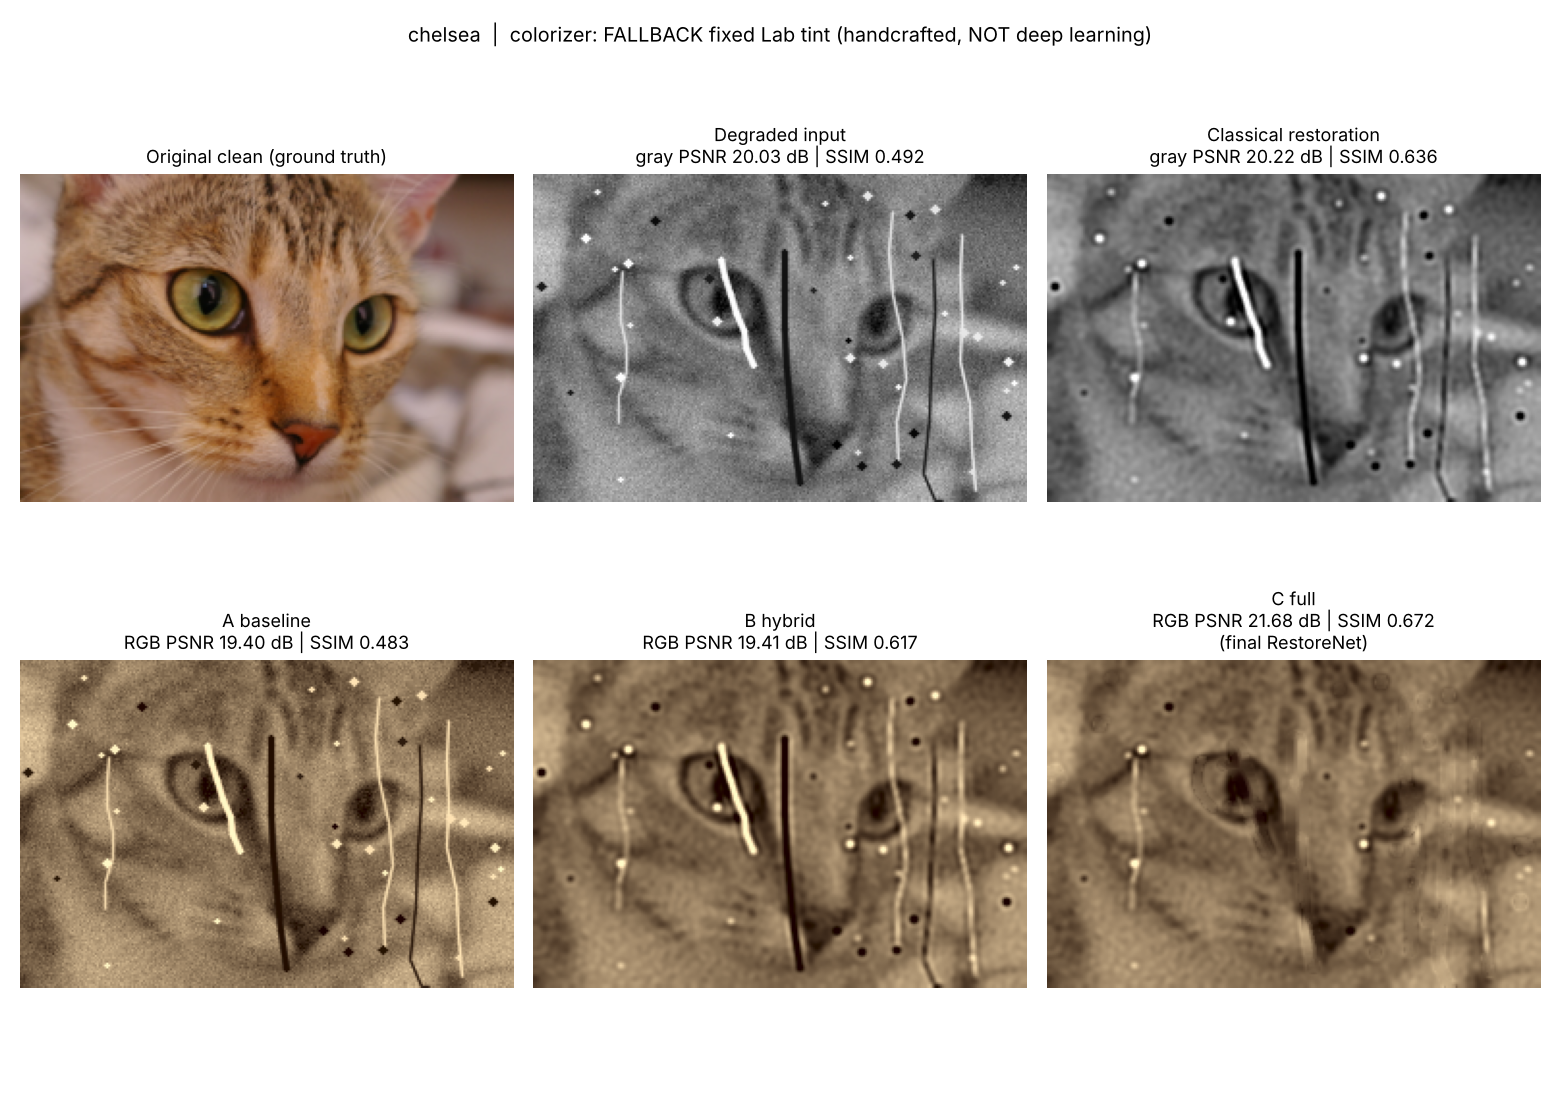
\includegraphics[width=\linewidth]{chelsea_comparison.png}
\caption{Qualitative comparison on one image (all panels resized to a common size). Ground truth, degraded input, classical output, and configurations A, B and C. Panel titles list measured metrics.}\label{fig:qual}
\end{figure}
\begin{figure}[t]\centering
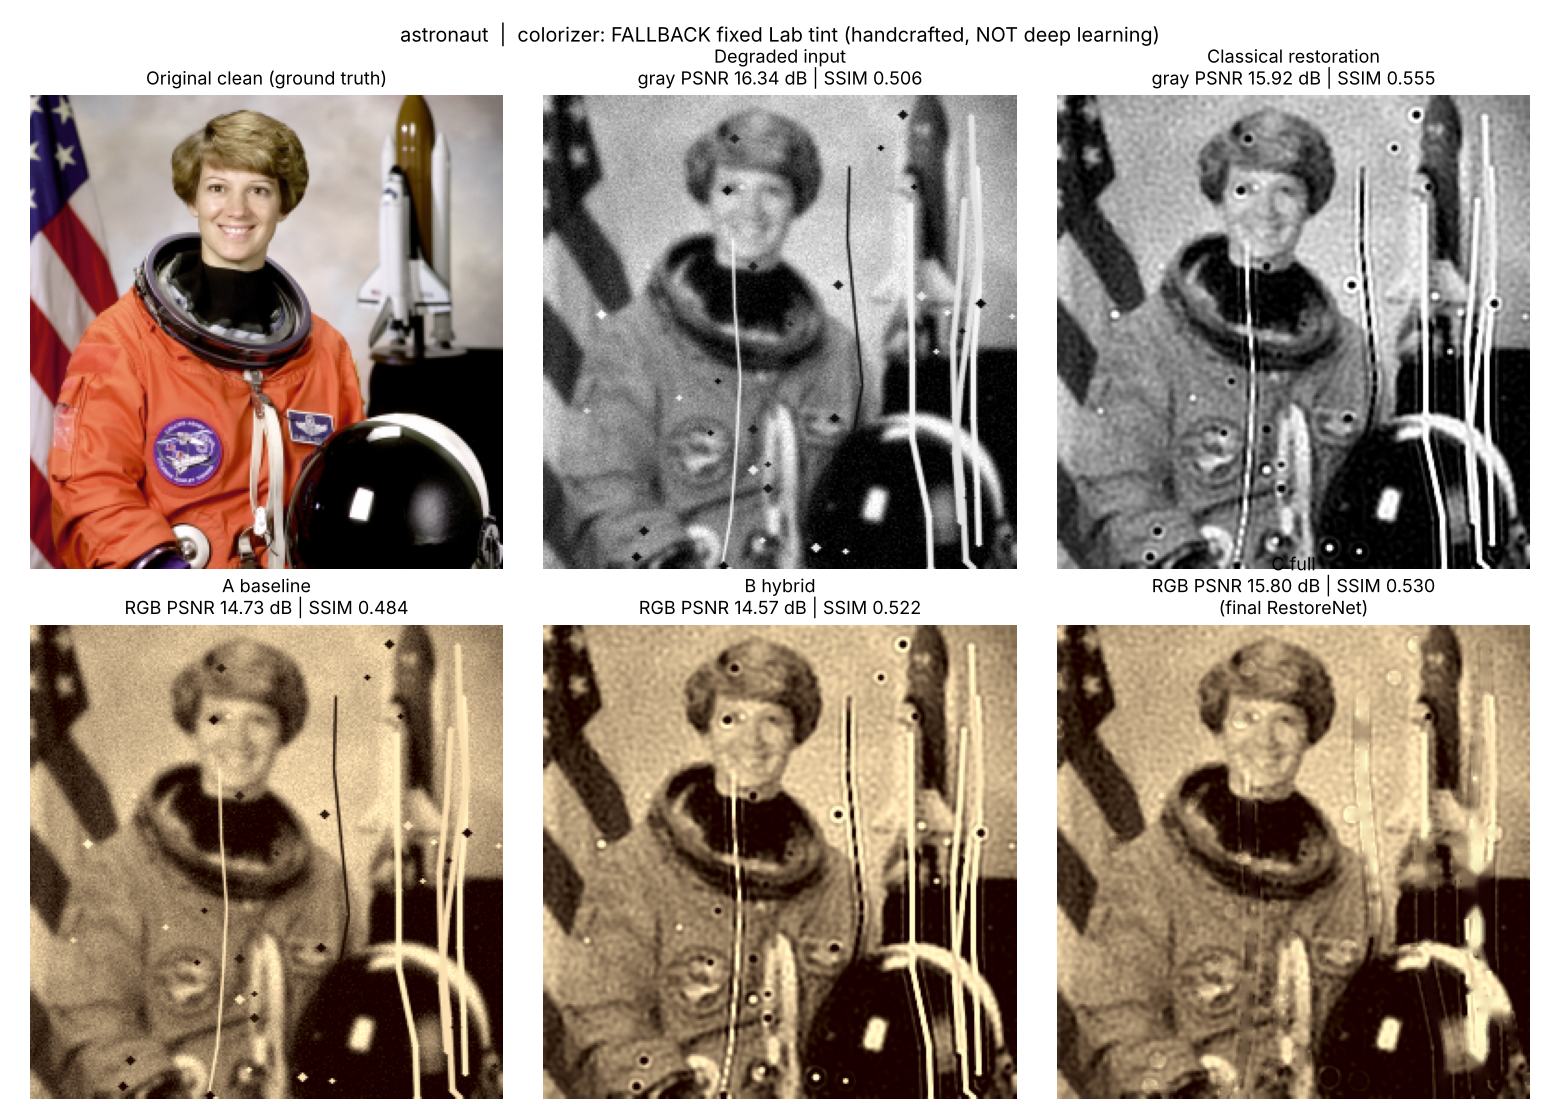
\includegraphics[width=\linewidth]{astronaut_comparison.png}
\caption{Second qualitative example.}\label{fig:qual2}
\end{figure}
\begin{figure}[t]\centering
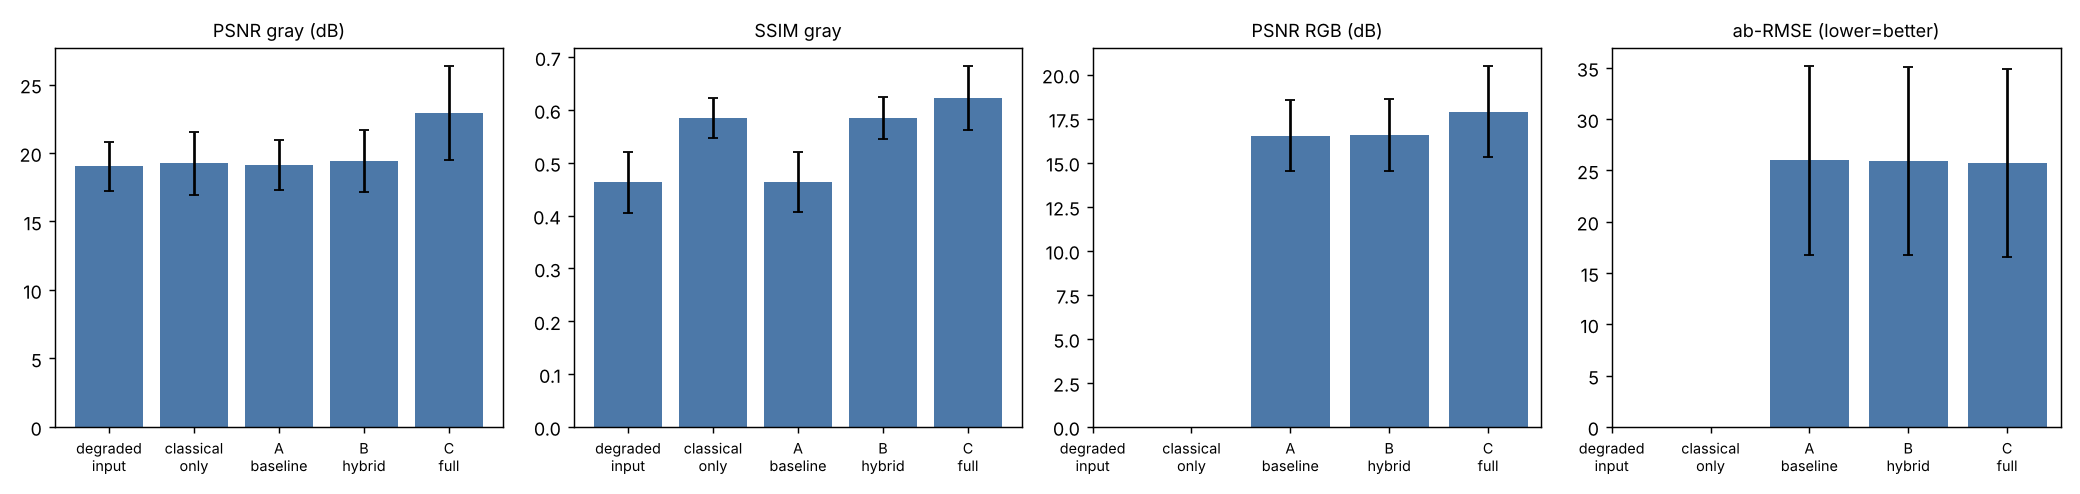
\includegraphics[width=\linewidth]{summary.png}
\caption{Mean metric per configuration (error bars: std over images).}\label{fig:summary}
\end{figure}
\begin{figure}[t]\centering
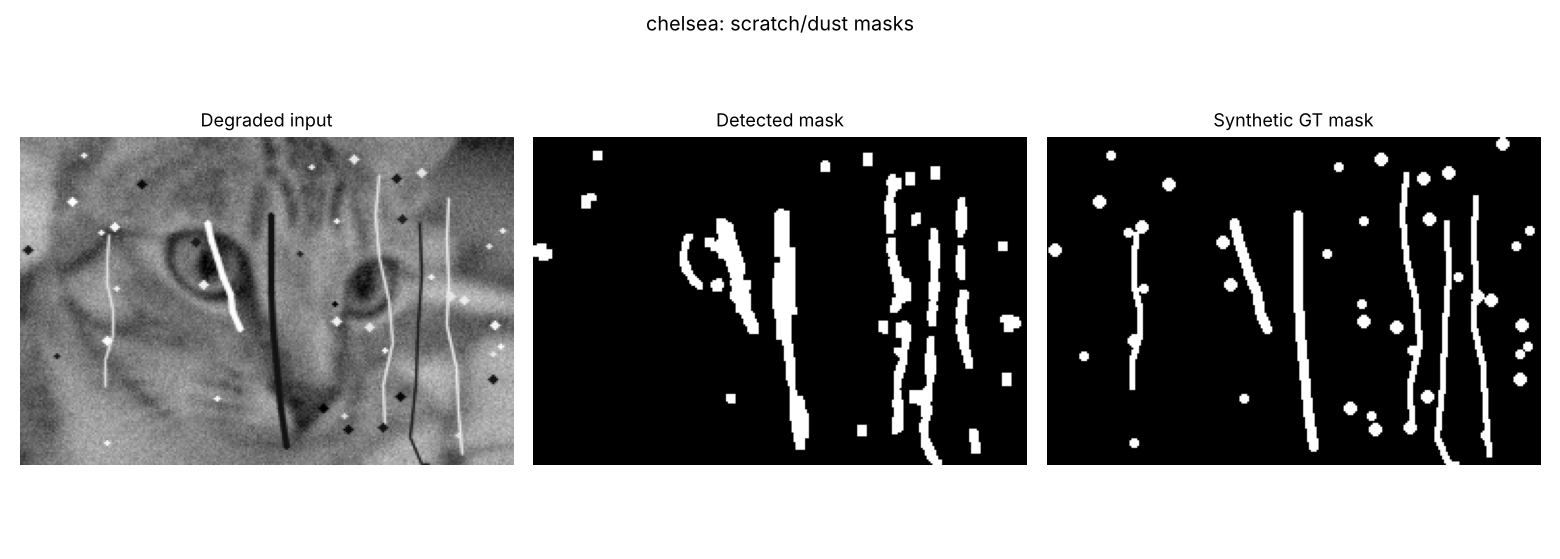
\includegraphics[width=0.9\linewidth]{chelsea_masks.png}
\caption{Detected mask vs.\ synthetic ground-truth mask.}\label{fig:masks}
\end{figure}
Visually (Fig.~\ref{fig:qual}), the classical stage visibly reduces noise but enlarges dust specks into blobs and leaves scratches, since both are high-contrast outliers rather than blur or Gaussian noise; the artifact-removal stage removes part of the scratches but misses some (Fig.~\ref{fig:masks}).
\todo{Re-check every qualitative and quantitative sentence in this section after the deep-colorizer run.}

\section{Ablation Study}
Table~\ref{tab:abl1} varies the classical stage (the colorized output is evaluated without artifact removal); Table~\ref{tab:abl2} varies the mask source, the inpainting method and the stage order.
In this run (see the tables for the exact numbers): the Wiener step alone gave \emph{lower} grayscale PSNR than no restoration, whereas median and Gaussian denoising raised it; Gaussian $\sigma=1$ gave the highest grayscale PSNR of the variants tried.
A sanity test on a blur-only image shows the Wiener implementation itself works, so with this noise level ($\sigma_n=10$) and mild blur ($\sigma=1.5$) a constant-$K$ Wiener filter simply amplifies noise more than it recovers detail; this does not say deblurring is useless in other regimes.
Oracle masks bound what detection can achieve; the automatic detector reaches the precision/recall in Table~\ref{tab:abl2}. Telea and Navier--Stokes behave almost identically. Running artifact removal \emph{before} the classical stage scored higher than the specified order (classical $\rightarrow$ colorize $\rightarrow$ artifact removal),
plausibly because Wiener/median processing spreads scratch energy before it can be masked; this is a hypothesis we did not test further. The $K$, PSF and order variants were evaluated on the same $\NImages$ images as the main results (no held-out set), so they are sensitivity analyses, not tuned improvements.

\section{Limitations}
(1) The deep colorizer was not run, so the core research question is unanswered by the reported numbers. (2) Only \NImages{} synthetic images, one degradation level, one seed; no confidence intervals or significance tests. (3) The Wiener PSF is the true synthetic PSF; real photographs need blind estimation.
(4) The scratch detector is heuristic with imperfect precision/recall, and synthetic scratches are simpler than real ones. (5) PSNR/SSIM against one original colour image do not measure colorization plausibility; LPIPS or user studies would be needed. (6) Timings are from a single-core sandbox and are only indicative.
(7) Synthetic degradation of a gray-converted modern photo is not the same as a genuine vintage photograph.

\section{Conclusion}
We built and ran a reproducible three-stage CPU pipeline and evaluation protocol. On our small synthetic benchmark, denoising and scratch removal improved measured fidelity, while Wiener deconvolution did not under noisy conditions,
and the stage order mattered. Whether classical restoration improves \emph{deep} colorization remains to be measured by re-running the provided pipeline with the pretrained weights.

\bibliographystyle{plainnat}
\bibliography{references}
\end{document}
